\documentclass[letterpaper,12pt]{article}
\usepackage{tabularx} % extra features for tabular environment
\usepackage{amsmath}  % improve math presentation
\usepackage{float}
\usepackage{pdfpages}

\usepackage{graphicx} % takes care of graphic including machinery
\graphicspath{ {./figures/} }
\usepackage[margin=1in,letterpaper]{geometry} % decreases margins
\usepackage{cite} % takes care of citations
\usepackage[final]{hyperref} % adds hyper links inside the generated pdf file
\hypersetup{
	colorlinks=true,       % false: boxed links; true: colored links
	linkcolor=blue,        % color of internal links
	citecolor=blue,        % color of links to bibliography
	filecolor=magenta,     % color of file links
	urlcolor =blue         
}




\begin{document}

\title{Experiment 2 Preliminary Work \protect\\ Miscellaneous Opamp Circuits}
\author{Ahmet Akman 2442366 \protect\\}
\date{\today}
\maketitle
\tableofcontents
%\begin{abstract}
%abstract
%\end{abstract}

%\section{Introduction}
\section{Step 1}

\begin{figure}[H]
    \centering
    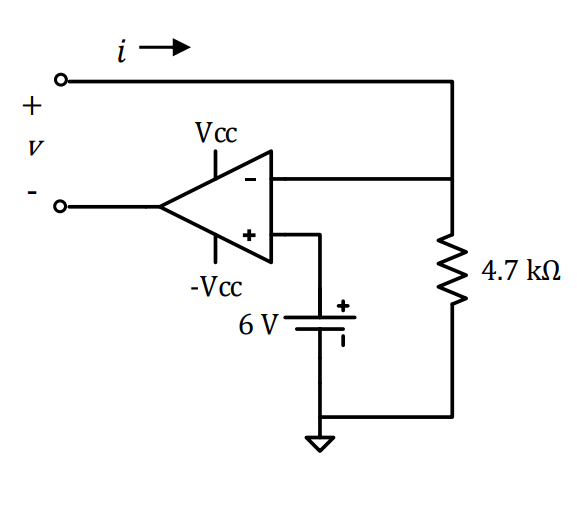
\includegraphics[width=0.65\textwidth]{1SCH.png}
\caption{Circuit schematic for the step 1}
\end{figure} 

\subsection{a)}

\subsection{b)}

\subsection{c)}
The simulation of the circuit given in Figure 1 is constructed in LTSpice environment. The schematic is given in Figure TODO .
\begin{figure}[H]
    \centering
    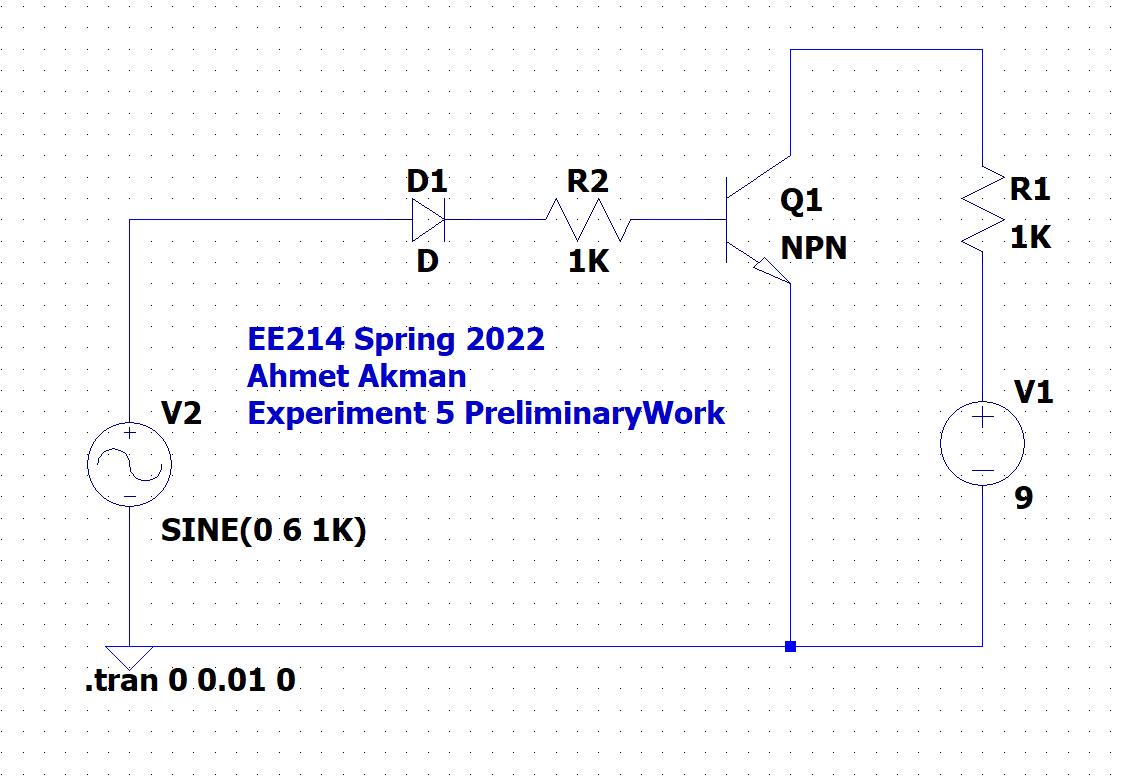
\includegraphics[width=1\textwidth]{1sim.png}
\caption{Circuit simulation schematic  for the step 1}
\end{figure} 
As a result, the plot given in Figure TODO is obtained.
\begin{figure}[H]
    \centering
    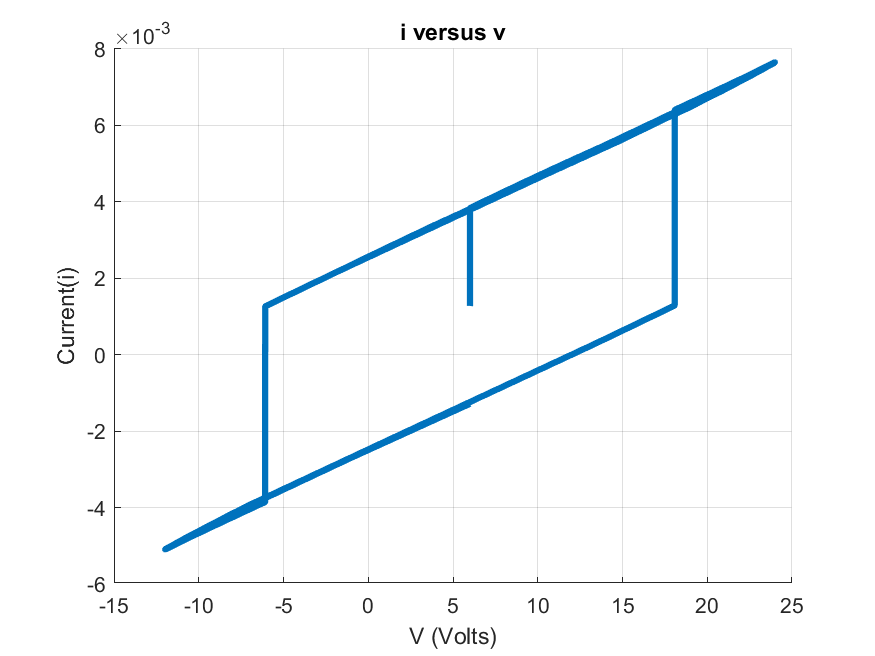
\includegraphics[width=1\textwidth]{1.png}
\caption{i versus v plot} 
\end{figure} 
\section{Step 2}

\begin{figure}[H]
    \centering
    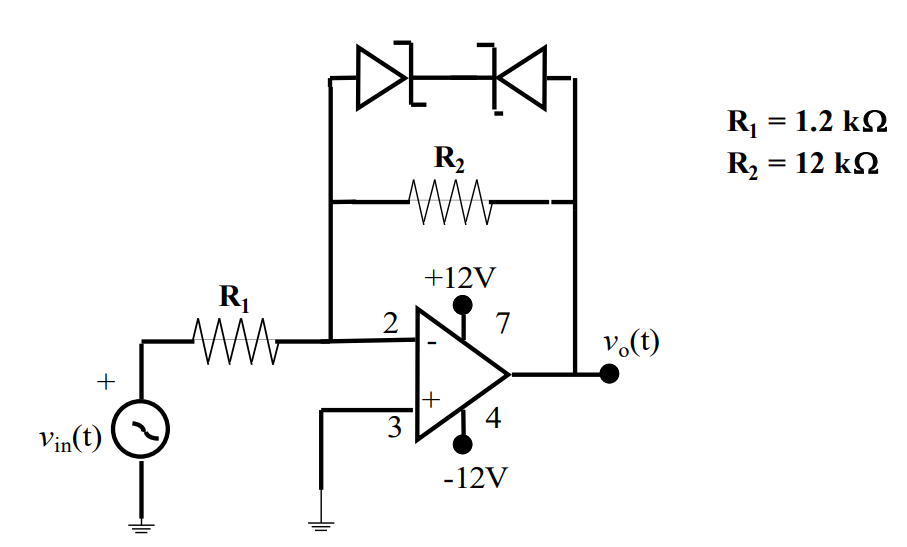
\includegraphics[width=0.65\textwidth]{2SCH.png}
\caption{Circuit schematic for the step 2}
\end{figure} 

The simulation of the circuit given in Figure TODO is constructed in LTSpice environment. The schematic is given in Figure TODO .
\begin{figure}[H]
    \centering
    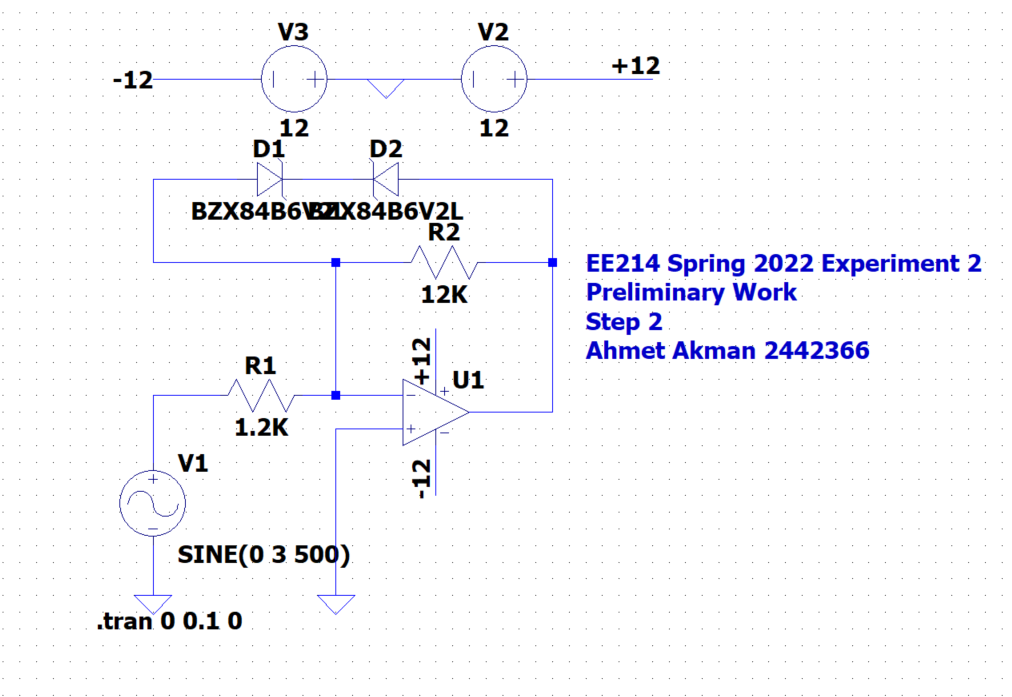
\includegraphics[width=1\textwidth]{2Sim.png}
\caption{Circuit simulation schematic  for the step 2}
\end{figure} 
As a result, the plot given in Figure TODO is obtained.
\begin{figure}[H]
    \centering
    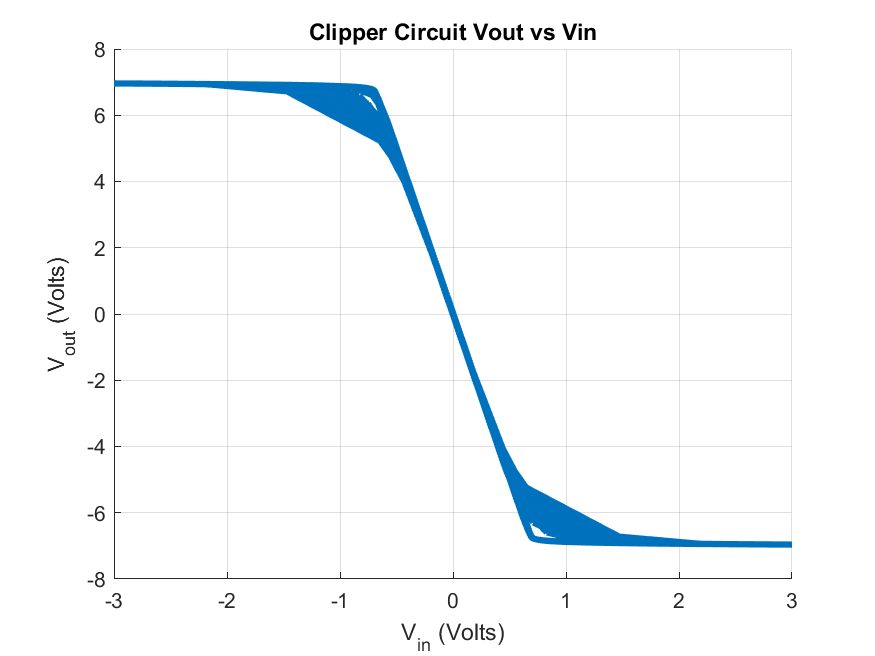
\includegraphics[width=1\textwidth]{2.png}
\caption{\(V_{in}\) and \(V_o\) versus time} 
\end{figure} 

\section{Step 3}


\begin{figure}[H]
    \centering
    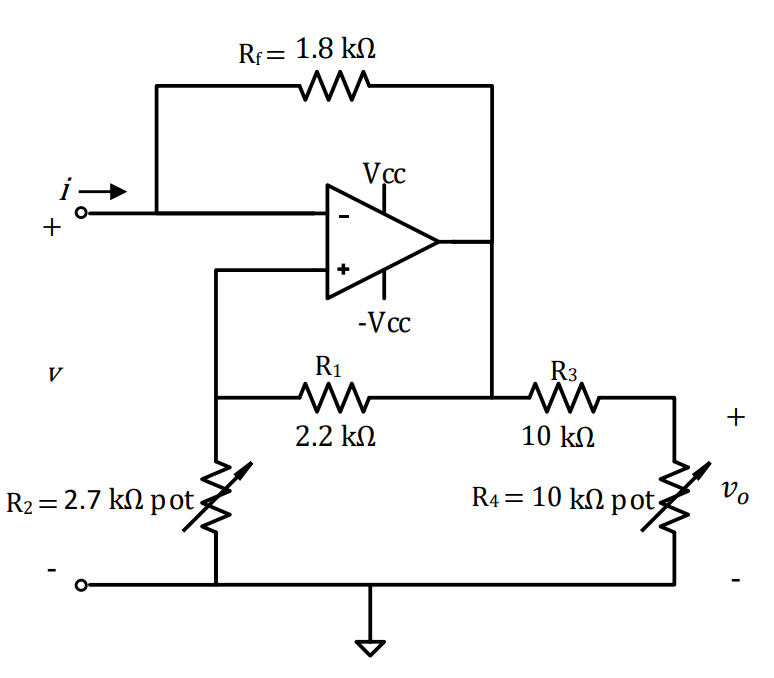
\includegraphics[width=0.65\textwidth]{3SCH.png}
\caption{Circuit schematic for the step 3}
\end{figure} 

\subsection{a)}
\subsection{b)}
\subsection{c)}
\subsection{d)}
The simulation of the circuit given in Figure TODO is constructed in LTSpice environment. The schematic is given in Figure TODO .
\begin{figure}[H]
    \centering
    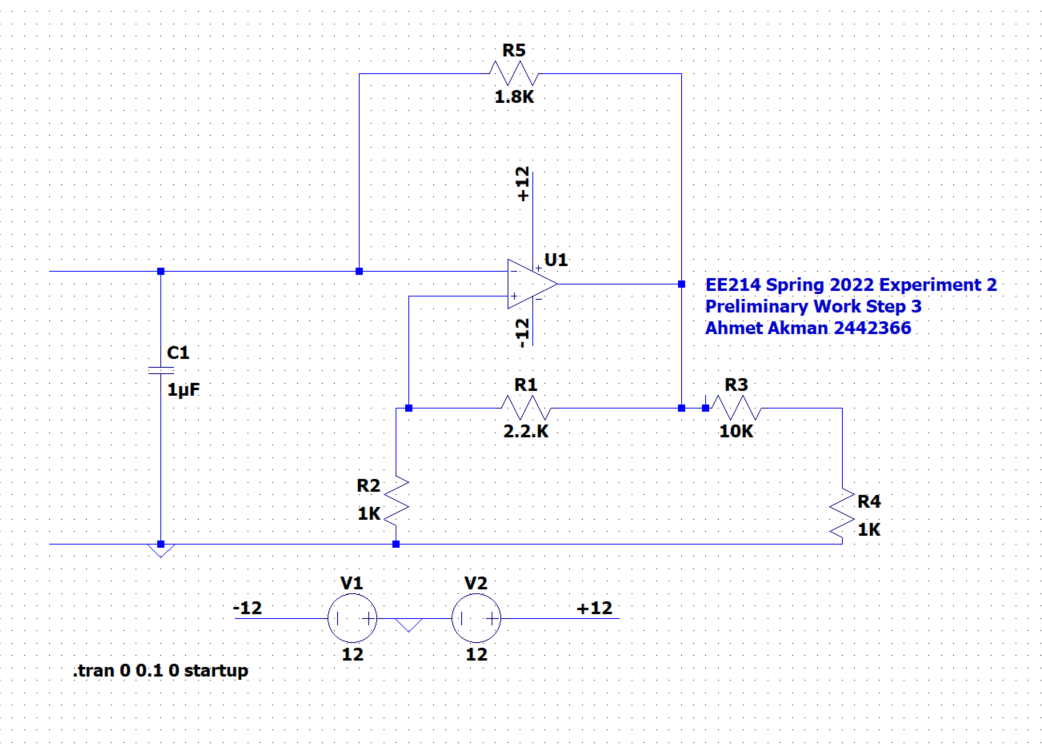
\includegraphics[width=1\textwidth]{3Sim.png}
\caption{Circuit simulation schematic  for the step 3}
\end{figure} 
As a result, the plot given in Figure TODO is obtained.
\begin{figure}[H]
    \centering
    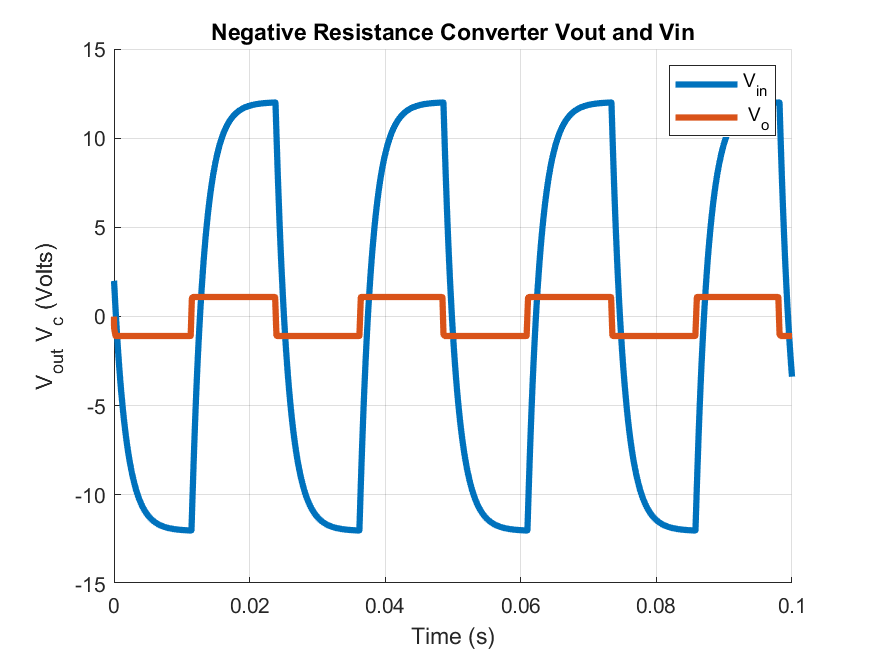
\includegraphics[width=1\textwidth]{3.png}
\caption{\(V_{in}\) and \(V_o\) versus time} 
\end{figure} 



\section{Conclusion}



\section*{Appendix A}
The results of the simulations are fetched from LTSpice and plotted in MATLAB in order to make the plots more readable and convenient.


\end{document}

%%%%%%%%%%%%%%%%%%%%%%   EXAMPLE TABLE   %%%%%%%%%%%%%%%%%%%%%%%%%%%%%%%%
\begin{table}[H]
\begin{center}
    \caption{Resistance reading by color code convention.}
    \vspace{2mm}
    \begin{tabular}{||c | c | c||} 
        \hline
        Color Order & Value & Tolerance \\ [0.5ex] 
        \hline\hline
        Brown / Black / Red / Gold & 1k\( \Omega \) & \( \% \) 5  \\ 
        \hline
        Yellow / Violet / Red / Gold & 4.7k\( \Omega \) & \( \% \) 5   \\
        \hline
        Brown / Grey / Orange / Gold & 18k\( \Omega \) & \( \% \) 5  \\ [1ex] 
        \hline
    \end{tabular}
\end{center}
\end{table}


%%%%%%%%%%%%%%%%%%%%%%   EXAMPLE IMAGE   %%%%%%%%%%%%%%%%%%%%%%%%%%%%%%%%
\begin{figure}[H]
\centering
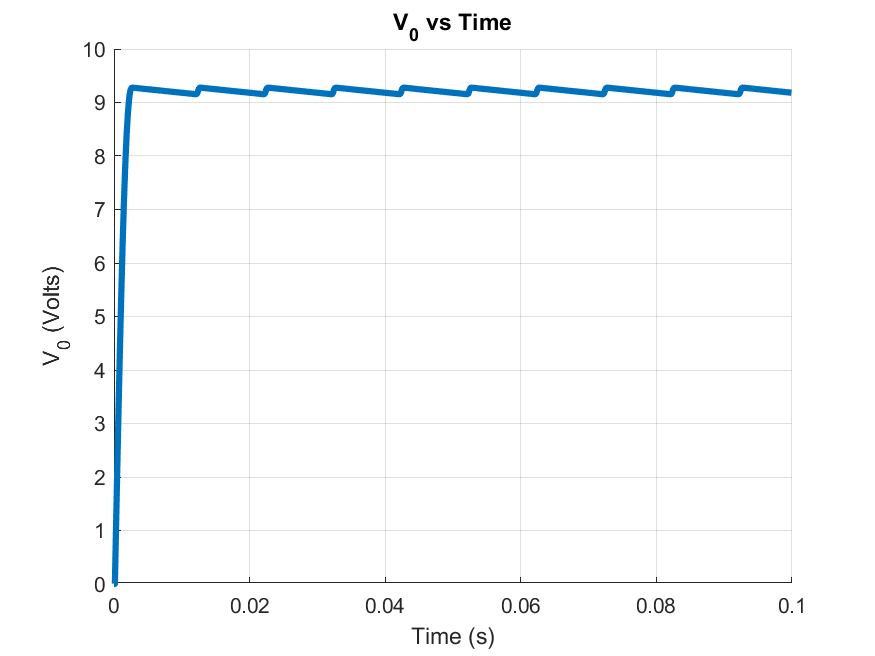
\includegraphics[width=1\textwidth]{5.png}
\caption{Circuit schematic for the step 5}
\end{figure} 

%%%%%%%%%%%%%%%%%%%%%%   EXAMPLE IMAGE FROM PDF   %%%%%%%%%%%%%%%%%%%%%%%%%%%%%%%%
\begin{figure}[H] \centering{
	\includegraphics[scale=0.25]{2a_plot.pdf}}
	\caption{Experiment 2}
\end{figure}
	